%; whizzy chapter
% -initex iniptex -latex platex -format platex -bibtex jbibtex -fmt fmt
% 以上 whizzytex を使用する場合の設定。

%     Kansai Debian Meeting resources
%     Copyright (C) 2007 Takaya Yamashita
%     Thank you for Tokyo Debian Meeting resources

%     This program is free software; you can redistribute it and/or modify
%     it under the terms of the GNU General Public License as published by
%     the Free Software Foundation; either version 2 of the License, or
%     (at your option) any later version.

%     This program is distributed in the hope that it will be useful,
%     but WITHOUT ANY WARRANTY; without even the implied warranty of
%     MERCHANTABILITY or FITNESS FOR A PARTICULAR PURPOSE.  See the
%     GNU General Public License for more details.

%     You should have received a copy of the GNU General Public License
%     along with this program; if not, write to the Free Software
%     Foundation, Inc., 51 Franklin St, Fifth Floor, Boston, MA  02110-1301 USA

%  preview (shell-command (concat "evince " (replace-regexp-in-string "tex$" "pdf"(buffer-file-name)) "&"))
% 画像ファイルを処理するためにはebbを利用してboundingboxを作成。
%(shell-command "cd image200708; ebb *.png")

%%ここからヘッダ開始。

\documentclass[mingoth,a4paper]{jsarticle}
\usepackage{kansaimonthlyreport}
\usepackage[dvips]{xy}
\usepackage{ulem}

% 日付を定義する、毎月変わります。
\newcommand{\debmtgyear}{2018}
\newcommand{\debmtgdate}{25}
\newcommand{\debmtgmonth}{3}
\newcommand{\debmtgnumber}{133}

\def\fixme#1{{\color{red}{#1}}}

\begin{document}

\begin{titlepage}

% 毎月変更する部分、本文の末尾も修正することをわすれずに

 第\debmtgnumber{}回 関西 Debian 勉強会資料

\vspace{2cm}

\begin{center}

\includegraphics{image200802/kansaidebianlogo.png}
\end{center}

\begin{flushright}
\hfill{}関西 Debian 勉強会担当者 佐々木・倉敷・のがた・かわだ・おおつき \\
\hfill{}\debmtgyear{}年\debmtgmonth{}月\debmtgdate{}日
\end{flushright}

\thispagestyle{empty}
\end{titlepage}

\dancersection{最近のDebian関係のイベント報告}{Debian JP}

\subsection{第132回関西Debian勉強会}
2 月 25 日に福島区民センターで開催されました。発表は西山和広さんによる「ufw 再入門」でした。 

\subsection{第161回東京エリアDebian勉強会}
3 月 24 日に新宿溝口クリニックで開催されました。発表は ysaito さんによる 「go/debian での機械学習環境構築について」

\begin{itemize}
		\item 現在、機械学習には R や python を利用することが標準的な選択肢です。
		\item 第三の選択肢として、go を利用した機械学習の実践、および、debian上でのデータバージョニング、パイプライン構築を例示します。
		\item 機械学習の個別のアルゴリズムには踏み込まず、環境構築についてポイントをお伝えします。
\end{itemize}

\dancersection{最近のDebian News}{Debian JP}

\subsection{2018/Mar/10th Stretch 9.4 がリリース}
\subsection{2018/Mar/16th Debian Conference 2018 registration 開始}
			call for parapers は 2018/June/18th https://debconf18.debconf.org/cfp/

\dancersection{事前課題}{関西Debian勉強会}

今回の事前課題はありませんでした。

参加者の皆さんは以下の通りです:
事前課題はありませんでした。

\begin{prework}{ ipv6waterstar }
\end{prework}

\begin{prework}{YukiharuYABUKI}
\end{prework}

\begin{prework}{ yosuke\_san }
\end{prework}

\begin{prework}{gdevmjc}
\end{prework}

\begin{prework}{sato\_makoto}
\end{prework}

\begin{prework}{nogajun}
\end{prework}

\begin{prework}{murase\_syuka}
\end{prework}

\begin{prework}{t3rkwd}
\end{prework}


\dancersection{我が家の仮想ネットワーク}{川江 浩}

\subsection{はじめに}
我が家のサーバ群の仮想ネットワークは、シンクライアントを前提に構築しています。シンクライアント(thin client)とは端末に最小限の処理をさせ、ほとんどの処理をサーバ側に集中させたシステムアーキテクチャ全般の事です。我が家ではqemu-kvm、qemuを使ってVM(Virtual Machine 以下VM)に各種サーバをインストールし運用しています。

ただし根本的な問題として、実PC上でqemu-kvmやqemuを使って複数のVMを走らせる事はサーバ、ネットワークの負荷を増大させ、VM自体のパフォーマンスも低下させます。また、データの共有や活用でも問題を生じます。そこで、逆説的な方法ですが、ローカルPC側でもVMを走らせ、仮想ネットワークを構築する事で以上の問題を軽減します。

また、以下の仕様はパーソナルベースでの運用を前提に構築したものです。仕様を試そうとするときは、必ずデータ等のバックアップをとって自己責任で行って下さい。より詳しく知りたい方は専門の書籍やセミナーなどを参考にしてください。

\subsection{仮想ネットワークの概要}
仮想ネットワークには、外部接続用サーバ、複数のVM、ローカルネットワークのみにつながっている複数の端末(タブレット等)があります。これらのマシンにサブネットで3つのブロック(192.168.24.0/25 192.168.24.128/26 192.168.24.192/26)に、分割したネットワークごとのプライベートIPアドレスを割り当て、利便性を確保します。具体的には
\begin{itemize}
\item 外部用ネットワーク\\
  外部用ネットワークはインターネットにつなぐため、PR-500MI(NTTのルータ)を使います。このルータは端末(実機、VMを問わず)のネットワークデバイスのMACアドレスを公開する事で、該当端末を直接インターネットにつなぐ事ができます。\\
  このルータの機能とDNSとして使うbindソフトウェアの各ステータスを利用して、各VMごとに192.168.24.0/25ブロックのプライベートIPアドレスを割り当て、1つのグローバルアドレスで複数の外部公開用VMを運用します。
\clearpage
\item 内部用ネットワーク\\
  内部用ネットワークは基本的にWifiでの接続を前提とします。さらに、実機のローカルPC自体は持ち運ぶのでテザリングでの接続もできるようにします。\\
  また、実際の作業やアプリケーションの活用はVMで行うので、ローカルPC自体には192.168.24.0/25のブロックのIPアドレスを、ローカルPC内で走るVMには更にサブネットマスクで2つに分けた、192.168.24.128/26のブロックと192.168.24.192/26のブロックのIPアドレスを割り当てます。
\end{itemize}
各ネットワークの設定は以下の通りです。

\subsection{外部用ネットワーク}
\subsubsection{外部用ネットワークの概要}
外部用ネットワークは、PR-500MIで外部ネットにつながり、第一義的なプライベートネットワークのセグメントを構成します。このセグメントでは外部公開用の各種サーバ、同セグメントのみアクセス可能なファイルサーバ、タブレット型PC、モバイル機器などがあり、これらをイーサネットやWifiで接続しています。

また、同セグメントに接続しているHand madeのrouterはさらに192.168.18.0/24のセグメントにつながっています(ただし、現在はSSHを使って、VMのホストPCを保守するのみ)。具体的なイメージは下図のようになります。

%図形の挿入
\begin{figure*}[!h]
\centering
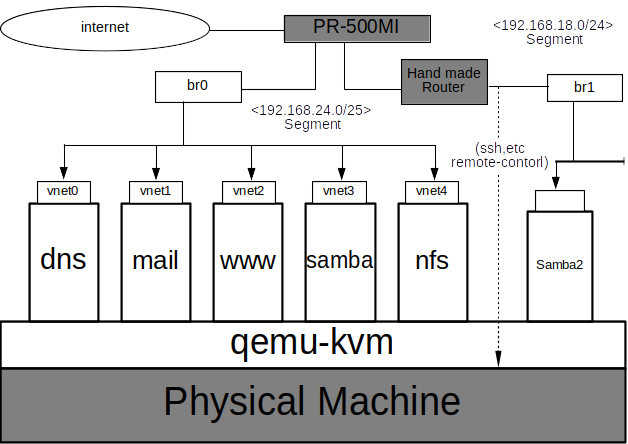
\includegraphics{image201803-kansai/external.png}
\caption{外部用ネットワークの図}
\end{figure*}
\clearpage

\subsubsection{外部用ネットワークの設定}
外部用のネットワークでの各VMのネットワークデバイスの設定は、第一にvirt-managerを使い仮想ネットワークを接続する仮想bridgeを作成します。次にVMのネットワークインターフェイスは、qemuでエミュレートされるTAPデバイスを作成して、単純に入出力を接続する「tap」を作ります。このtapは擬似的なethernetデバイスでLinuxカーネルの機能です。この仮想的なethernetデバイスを、同じくLinuxのカネールの機能である仮想bridgeで接続するこで、VMは実デバイスやほかのVMと接続することができます。

ただし、virt-managerで作成する仮想bridgeはdefaultでサブネットを設定できません。なので、interfacesファイルを直接、編集してサブネットを設定します。また、Hand made Router、VMのDNSの両方にbindパッケージをインストールし、外部用ネットワークを構築します。

次に、Hand made Routerはルータにするために、iptablesとiptables-persistenのパッケージを使います。また、/etc/sysctl.confのnet.ipv4.ip_forward=1のコメントを外しておきます。具体的には

\begin{itemize}
\item 仮想bridge、Hand made Routerでのサブネットの設定\\
VMを走らせる実機は qemu-kvm virt-managerをインストールして設定します。そして同機の/etc/network/interfacesを以下のように直接、編集します。
\begin{commandline}
# The loopback network interface
auto lo
iface lo inet loopback

# The primary network interface
allow-hotplug br0
iface br0 inet static
   address 192.168.24.108
   netmask 255.255.255.128
   gateway 192.168.24.1
   bridge_ports enp9s0
   bridge_stp on
   bridge_fd 0.0
# This is an autoconfigured IPv6 interface
iface enp9s0 inet6 auto

# The secondary network interface
auto enx0022cf56e5ca
allow-hotplug enx0022cf56e5ca
iface enx0022cf56e5ca inet static
address 192.168.18.80
netmask 255.255.255.0
gateway 192.168.18.80
# This is an autoconfigured IPv6 interface
iface enx0022cf56e5ca inet6 auto
\end{commandline}
次にHand made Routerはルータとして機能し、VMのモニターと保守も行い、インターネットからの入口にもします。設定としては /etc/network/interfacesと/etc/iptables/rules.v4を以下の様にします。\\
--------interfaces--------
\begin{commandline}
# The loopback network interface
auto lo
iface lo inet loopback

# The primary network interface
auto enp2s1
allow-hotplug enp2s1
iface enp2s1 inet static
address 192.168.24.88
netmask 255.255.255.128
gateway 192.168.24.1

# This is an autoconfigured IPv6 interface
iface enp2s1 inet6 auto

# The secondary network interface
allow-hotplug ens32
iface ens32 inet static
address 192.168.18.1
netmask 255.255.255.0
gateway 192.168.18.1

# This is an autoconfigured IPv6 interface
iface ens32 inet6 auto
\end{commandline}
\clearpage
--------rules.v4--------
\begin{commandline}
# Generated by iptables-save v1.6.0 on Sat Nov 18 17:30:00 2017
*filter
:INPUT ACCEPT [0:0]
:FORWARD ACCEPT [0:0]
:OUTPUT ACCEPT [0:0]

-A INPUT -i lo -j ACCEPT
...(Omltted)...
-A INPUT -i enp2s1 -m state --state RELATED,ESTABLISHED -j ACCEPT
-A INPUT -i enp2s1 -j DROP
...(Omltted)...
-A FORWARD -o ens32 -j REJECT --reject-with icmp-port-unreachable
-A FORWARD -i enp2s1 -m state --state RELATED,ESTABLISHED -j ACCEPT
-A FORWARD -o ens32 -m state --state NEW,ESTABLISHED -j ACCEPT

-A FORWARD -i enp2s1 -j DROP
-A FORWARD -o ens32 -j DROP

-A OUTPUT -o lo -j ACCEPT
...(Omltted)...
-A OUTPUT -o ens32 -m state --state NEW,ESTABLISHED -j ACCEPT
-A OUTPUT -o ens32 -j DROP
COMMIT
# Completed on Sat Mar 25 17:12:38 2017

# Generated by iptables-save v1.6.0 on Sat Apr 29 10:00:07 2017
*mangle
:PREROUTING ACCEPT [0:0]
:INPUT ACCEPT [0:0]
:FORWARD ACCEPT [0:0]
:OUTPUT ACCEPT [0:0]
:POSTROUTING ACCEPT [0:0]
-A POSTROUTING -o ens32 -p udp -m udp --dport 68 -j CHECKSUM --checksum-fill
COMMIT
# Completed on Sat Aug 26 16:07:34 2017

# Generated by iptables-save v1.4.21 on Sat Aug 26 16:07:34 2017
*nat
:PREROUTING ACCEPT [0:0]
:INPUT ACCEPT [0:0]
:OUTPUT ACCEPT [0:0]
:POSTROUTING ACCEPT [0:0]

-A POSTROUTING -s 192.168.18.0/24 ! -d 192.168.18.0/24 -j SNAT --to-source 192.168.24.88
COMMIT
# Completed on Sat Nov 18 17:30:00 2017  
\end{commandline}

\clearpage

\item bindの各ステータスを使った外部用ネットワークの設定\\
 VMのDNS、Hand Made Routerにインストールするbindパッケージのnamed.confの設定方法は下図の通り。概要としては設定ファイルのnamed.confにincludeステーメントを使い、aclステートメント、optionsステートメントの設定ファイルを挿入します。同様にviewステートメントで、条件付けファイルによる動作を定義し、includeステートメントで条件ファイルを挿入します。
%図形の挿入
\begin{figure*}[!h]
\centering
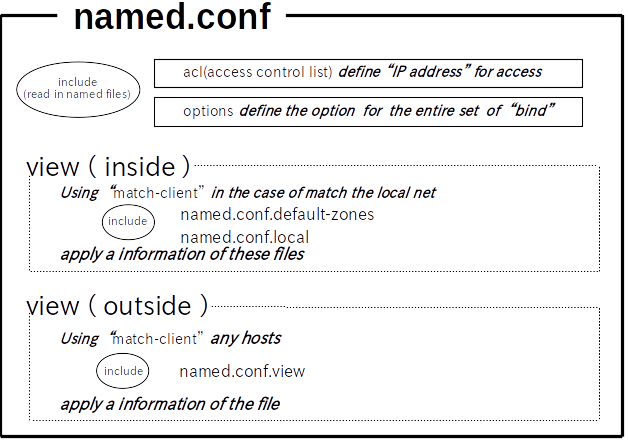
\includegraphics{image201803-kansai/named_conf.png}
\caption{named.confの図}
\end{figure*}

以下、各設定ファイルの詳細です。
\clearpage

\item named.conf(bindの設定ファイル)
\begin{commandline}
// This is the primary configuration file for the BIND DNS server named.
//
// Please read /usr/share/doc/bind9/README.Debian.gz for information on the 
// structure of BIND configuration files in Debian, *BEFORE* you customize 
// this configuration file.
//
// If you are just adding zones, please do that in /etc/bind/named.conf.local

include "/etc/bind/named.conf.acl";
include "/etc/bind/named.conf.options";

view "internal"{
	match-clients { localnet; };
	recursion yes;

include "/etc/bind/named.conf.local";
include "/etc/bind/named.conf.default-zones";

};

view "external" {
	match-clients { any; };
	recursion no;

include "/etc/bind/named.conf.view";

};    
\end{commandline}
各ステートメントごとの設定ファイルは以下のようになります。\\

\item aclステートメント(アクセスするネットワークのIPアドレスの設定ファイル)
\begin{commandline}
acl localnet{ 
	192.168.24.0/25;
	192.168.24.128/26;
	192.168.24.192/26;
	192.168.18.0/24; 
	127.0.0.1; 
};
\end{commandline}

\item optionsステートメント(オプションでbind全体の動作を設定する)
\begin{commandline}
options {
	directory "/var/cache/bind";

	// If there is a firewall between you and nameservers you want
	// to talk to, you may need to fix the firewall to allow multiple
	// ports to talk.  See http://www.kb.cert.org/vuls/id/800113

	// If your ISP provided one or more IP addresses for stable 
	// nameservers, you probably want to use them as forwarders.  
	// Uncomment the following block, and insert the addresses replacing 
	// the all-0's placeholder.

	forwarders {
	 	8.8.8.8; 8.8.4.4;
	};

	//========================================================================
	// If BIND logs error messages about the root key being expired,
	// you will need to update your keys.  See https://www.isc.org/bind-keys
	//========================================================================
	dnssec-validation auto;
	allow-query { any; };
        allow-transfer{ 
		localnet;
		8.8.8.8;
		8.8.4.4; 
	};
	version "no version";
	auth-nxdomain no;    # conform to RFC1035
	listen-on-v6 { any; };
};
\end{commandline}
\clearpage

\item viweステートメント(内部)\\
  match-clientを使いローカルネットに以下の設定ファイルを適用する。\\
--- named.conf.default-zone ---
\begin{commandline}
// prime the server with knowledge of the root servers
zone "." {
	type hint;
	file "/etc/bind/db.root";
};

// be authoritative for the localhost forward and reverse zones, and for
// broadcast zones as per RFC 1912

zone "localhost" {
	type master;
	file "/etc/bind/db.local";
};

zone "127.in-addr.arpa" {
	type master;
	file "/etc/bind/db.127";
};

zone "0.in-addr.arpa" {
	type master;
	file "/etc/bind/db.0";
};

zone "255.in-addr.arpa" {
	type master;
	file "/etc/bind/db.255";
};
\end{commandline}
zoneステートメント(ホスト名とIPアドレスの対応関係のリストを定義する)で使われているこれらのファイルはdefaultでbindフォルダに含まれています。\\
--- named.conf.local ---
\begin{commandline}
//
// Do any local configuration here
//
zone "kinsen.gr.jp" {
	type master;
	file "/etc/bind/db.in-kinsen.gr.jp";
};
zone "24.168.192.in-addr.arpa" {
	type master;
	file "/etc/bind/db.192.168.24";
};
zone "18.168.192.in-addr.arpa" {
	type master;
	file "/etc/bind/db.192.168.18";
};
// Consider adding the 1918 zones here, if they are not used in your
// organization
//include "/etc/bind/zones.rfc1918";
\end{commandline}
以上のファイルは以下の通りです。
\clearpage

--- db.in-kinsen.gr.jp ---
\begin{commandline}
;
; BIND data file for kinsen.gr.jp
;
$TTL	86400
@	IN     SOA      bandai.kinsen.gr.jp. root.bandai.kinsen.gr.jp. (
		              1         ; Serial
			   1800         ; Refresh
			    900         ; Retry
			 604800         ; Expire
			   1200 )       ; Negative Cache TTL

		IN      NS      dns

; localhost
localhost       IN      A       127.0.0.1
localhost       IN      AAAA    ::1

; Mail exchange
                IN      MX      0 mail.kinsen.gr.jp.
;
; Host entry
;
mizu0           IN      A       192.168.18.1
;               IN      AAAA    2001
mizu1           IN      A       192.168.18.2
;               IN      AAAA    2001
kamaba          IN      A       192.168.18.80
;               IN      AAAA    2001
noren           IN      A       192.168.24.108
;               IN      AAAA    2001
dns             IN      A       192.168.24.81
;               IN      AAAA    2001:
mail            IN      A       192.168.24.82
;               IN      AAAA    2001:
www             IN      A       192.168.24.83
;               IN      AAAA    2001:
karan           IN      A       192.168.24.84
;               IN      AAAA    2001:
datuiba         IN      A       192.168.24.85
;               IN      AAAA    2001:
bandai          IN      A       192.168.24.88
;               IN      AAAA    2001:
yubune          IN      A       192.168.24.18
;               IN      AAAA    2001:
;
; Alias
;www            IN      CNAME    noren
;
; Domain
@               IN      A       192.168.24.88
                IN      MX 0    mail
\end{commandline}
--- db.192.168.24 ---
\begin{commandline}
;
; BIND data file for 192.168.24 network
;
$TTL	86400
@         IN    SOA     bandai.kinsen.gr.jp. root.bandai.kinsen.gr.jp. (
		              1         ; Serial
			   1800         ; Refresh
			    900         ; Retry
			 604800         ; Expire
			   1200 )       ; Negative Cache TTL

                IN      NS      dns
;
; Host entry
;
108             IN      PTR     noren.kinsen.gr.jp.
81              IN      PTR     dns.kinsen.gr.jp.
82              IN      PTR     mail.kinsen.gr.jp.
83              IN      PTR     www.kinsen.gr.jp.
84              IN      PTR     karan.kinsen.gr.jp.
85              IN      PTR     datuiba.kinsen.gr.jp.
88              IN      PTR     bandai.kinsen.gr.jp.
18              IN      PTR     yubune.kinsen.gr.jp.
\end{commandline}
\clearpage

\item viewステートメント(外部)\\
  match-clientを使いすべての外部hostにnamed.conf.viewファイルを適用する。\\
--- named.conf.view ---
\begin{commandline}
zone "." {
	type hint;
	file "/etc/bind/db.root";
};
zone "kinsen.gr.jp"{
	type master;
	file "/etc/bind/db.out-kinsen.gr.jp";
};
zone "158.141.203.in-addr.arpa"{
	type master;
	file "/etc/bind/db.203.141.158";
};    
\end{commandline}
db.rootファイルはdefaultでbindフォルダにあります。out-kinsen.gr.jp、db.203.141.158については以下の通り。\\
--- out-kinsen.gr.jp ---
\begin{commandline}
;
; BIND data file for kinsen.gr.jp
;
$TTL	86400
@        IN      SOA    bandai.kinsen.gr.jp. root.bandai.kinsen.gr.jp. (
                              1         ; Serial
			   1800         ; Refresh
			    900         ; Retry
			 604800         ; Expire
			   1200 )       ; Negative Cache TTL
                                   
                IN   NS       dns

; localhost
localhost       IN      A       127.0.0.1
localhost       IN      AAAA    ::1

; Mail exchange
                IN      MX      0 mail.kinsen.gr.jp.
;
; Host entry
;
noren           IN      A       203.141.158.41
;               IN      AAAA    2001:
dns             IN      A       203.141.158.41
;               IN      AAAA    2001:
mail            IN      A       203.141.158.41
;               IN      AAAA    2001:
www             IN      A       203.141.158.41
;               IN      AAAA    2001:
karan           IN      A       203.141.158.41
;               IN      AAAA    2001:
datuiba         IN      A       203.141.158.41
;               IN      AAAA    2001:
bandai          IN      A       203.141.158.41
;               IN      AAAA    2001:
yubune          IN      A       203.141.158.41
;               IN      AAAA    2001:
;
; Domain
@               IN      A       203.141.158.41
                IN      MX 0    mail
\end{commandline}
\clearpage

--- db.203.141.58 ---
\begin{commandline}
;
; BIND data file for 203.141.158 network
;
$TTL    86400
@       IN      SOA     bandai.kinsen.gr.jp. root.bandai.kinsen.gr.jp. (
                              1         ; Serial
                           1800         ; Refresh
                            900         ; Retry
                         604800         ; Expire
                           1200 )       ; Negative Cache TTL

                  IN        NS      dns
;
; Host entry
;
41		IN	PTR	noren.kinsen.gr.jp.
41		IN	PTR	dns.kinsen.gr.jp.
41		IN	PTR	mail.kinsen.gr.jp.
41		IN	PTR	www.kinsen.gr.jp.
41		IN	PTR	karan.kinsen.gr.jp.
41		IN	PTR	datuiba.kinsen.gr.jp.
41		IN	PTR	bandai.kinsen.gr.jp.
41		IN	PTR	yubune.kinsen.gr.jp.
\end{commandline}
\end{itemize}

\subsection{内部用ネットワーク}
\subsubsection{内部用ネットワークの概要}
内部用ネットワークは実機PCに仮想ルータを作り、Wifi経由で実機上で走るVMをプライベートネットを3に分けたそれぞれのセグメント(192.168.24.0/25 192.168.24.128/26 1923168.24.192/26)につなぎます。\\
概要は下図の通り。

%図形の挿入
\begin{figure*}[!h]
\centering
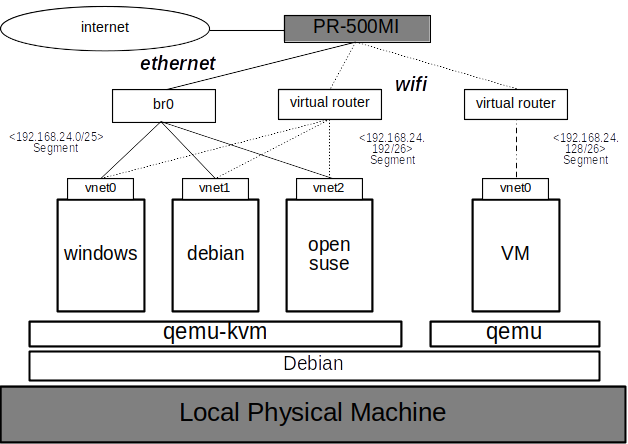
\includegraphics{image201803-kansai/internal.png}
\caption{内部用ネットワークの図}
\end{figure*}
\clearpage

\subsubsection{内部用ネットワークの設定}
内部用ネットワークの設定は、前提としてvirt-managerのConnection Detailsのvirtual networkで仮想ルータを作っておきます。また、実機PCをルータにする事を前提にしていますので、前述のHand made Routerのように、interfacesとrules.v4のファイルを以下のように設定します。

--- interfaces ---
\begin{commandline}
# This file describes the network interfaces available on your system
# and how to activate them. For more information, see interfaces(5).

source /etc/network/interfaces.d/*

# The loopback network interface
auto lo
iface lo inet loopback

# The primary network interface
allow-hotplug wlp1s0
iface  wlp1s0 inet dhcp

# This is an autoconfigured IPv6 interface
iface wlp1s0 inet6 auto

# The primary network interface
allow-hotplug enx0022cf56e5ca
iface br0 inet static
   address 192.168.24.8
   netmask 255.255.255.128
   gateway 192.168.24.1
   bridge_ports enx0022cf56e5ca
   bridge_stp on
   bridge_fd 0.0
# This is an autoconfigured IPv6 interface
iface enx0022cf56e5ca inet6 auto
iface br0 inet6 auto
\end{commandline}
\clearpage

--- rules.v4 ---
\begin{commandline}
# Generated by iptables-save v1.6.0 on Sat Apr 29 10:00:07 2017
*filter
:INPUT ACCEPT [0:0]
:FORWARD ACCEPT [0:0]
:OUTPUT ACCEPT [0:0]
-A INPUT -i lo -j ACCEPT
-A INPUT -i enx0022cf56e5ca -j ACCEPT
-A INPUT -i br0 -j ACCEPT

-A INPUT -i wlp1s0 -p udp -m udp --dport 123 -j ACCEPT
-A INPUT -i wlp1s0 -p udp -m udp --dport 53 -j ACCEPT
-A INPUT -i wlp1s0 -p tcp -m tcp --dport 53 -j ACCEPT
-A INPUT -i wlp1s0 -p udp -m udp --dport 67:68 -j ACCEPT
-A INPUT -i wlp1s0 -p tcp -m tcp --dport 80 -j ACCEPT
-A INPUT -i wlp1s0 -p tcp -m tcp --dport 443 -j ACCEPT
-A INPUT -i wlp1s0 -p udp -m udp --dport 111 -j ACCEPT
-A INPUT -i wlp1s0 -p tcp -m tcp --dport 111 -j ACCEPT
-A INPUT -i wlp1s0 -p udp -m udp --dport 2049 -j ACCEPT
-A INPUT -i wlp1s0 -p tcp -m tcp --dport 2049 -j ACCEPT
-A INPUT -i wlp1s0 -p udp -m udp --dport 445 -j ACCEPT
-A INPUT -i wlp1s0 -p tcp -m tcp --dport 445 -j ACCEPT
-A INPUT -i wlp1s0 -p tcp -m tcp --dport 5900:6000 -j ACCEPT
-A INPUT -i wlp1s0 -p udp -m udp --dport 32800:32805 -j ACCEPT
-A INPUT -i wlp1s0 -p tcp -m tcp --dport 32800:32805 -j ACCEPT
-A INPUT -i wlp1s0 -m state --state RELATED,ESTABLISHED -j ACCEPT
-A INPUT -i wlp1s0 -j DROP


-A FORWARD -i wlp1s0 -p udp -m udp --dport 123 -j ACCEPT
-A FORWARD -o virbr1 -p udp -m udp --sport 123 -m state --state ESTABLISHED -j ACCEPT
-A FORWARD -i wlp1s0 -p udp -m udp --dport 53 -j ACCEPT
-A FORWARD -o virbr1 -p udp -m udp --sport 53 -m state --state ESTABLISHED -j ACCEPT
-A FORWARD -i wlp1s0 -p tcp -m tcp --dport 53 -j ACCEPT
-A FORWARD -o virbr1 -p tcp -m tcp --sport 53 -m state --state ESTABLISHED -j ACCEPT
-A FORWARD -i wlp1s0 -p udp -m udp --dport 67 -j ACCEPT
-A FORWARD -o virbr1 -p udp -m udp --sport 67 -m state --state ESTABLISHED -j ACCEPT
-A FORWARD -i wlp1s0 -p udp -m udp --dport 68 -j ACCEPT
-A FORWARD -o virbr1 -p udp -m udp --sport 68 -m state --state ESTABLISHED -j ACCEPT
-A FORWARD -i wlp1s0 -p tcp -m tcp --dport 80 -j ACCEPT
-A FORWARD -o virbr1 -p tcp -m tcp --sport 80 -m state --state ESTABLISHED -j ACCEPT
-A FORWARD -i wlp1s0 -p tcp -m tcp --dport 443 -j ACCEPT
-A FORWARD -o virbr1 -p tcp -m tcp --sport 443 -m state --state ESTABLISHED -j ACCEPT
-A FORWARD -i wlp1s0 -p udp -m udp --dport 445 -j ACCEPT
-A FORWARD -o virbr1 -p udp -m udp --sport 445 -m state --state ESTABLISHED -j ACCEPT
-A FORWARD -i wlp1s0 -p tcp -m tcp --dport 445 -j ACCEPT
-A FORWARD -o virbr1 -p tcp -m tcp --sport 445 -m state --state ESTABLISHED -j ACCEPT
-A FORWARD -i wlp1s0 -p tcp -m tcp --dport 5900:6000 -j ACCEPT
-A FORWARD -o virbr1 -p tcp -m tcp --sport 5900:6000 -m state --state ESTABLISHED -j ACCEPT
-A FORWARD -o virbr1 -j REJECT --reject-with icmp-port-unreachable
-A FORWARD -i wlp1s0 -m state --state RELATED,ESTABLISHED -j ACCEPT
-A FORWARD -o virbr1 -m state --state NEW,ESTABLISHED -j ACCEPT
-A FORWARD -i wlp1s0 -j DROP
-A FORWARD -o virbr1 -j DROP

-A OUTPUT -o lo -j ACCEPT
-A OUTPUT -o br0 -j ACCEPT

-A OUTPUT -o virbr1 -p udp -m udp --sport 123 -j ACCEPT
-A OUTPUT -o virbr1 -p udp -m udp --sport 53 -j ACCEPT
-A OUTPUT -o virbr1 -p tcp -m tcp --sport 53 -j ACCEPT
-A OUTPUT -o virbr1 -p udp -m udp --sport 67:68 -j ACCEPT
-A OUTPUT -o virbr1 -p tcp -m tcp --sport 80 -j ACCEPT
-A OUTPUT -o virbr1 -p tcp -m tcp --sport 443 -j ACCEPT
-A OUTPUT -o virbr1 -p udp -m udp --sport 111 -j ACCEPT
-A OUTPUT -o virbr1 -p tcp -m tcp --sport 111 -j ACCEPT
-A OUTPUT -o virbr1 -p udp -m udp --sport 2049 -j ACCEPT
-A OUTPUT -o virbr1 -p tcp -m tcp --sport 2049 -j ACCEPT
-A OUTPUT -o virbr1 -p udp -m udp --sport 445 -j ACCEPT
-A OUTPUT -o virbr1 -p tcp -m tcp --sport 445 -j ACCEPT
-A OUTPUT -o virbr1 -p tcp -m tcp --sport 5900:6000 -j ACCEPT
-A OUTPUT -o virbr1 -p udp -m udp --sport 32800:32805 -j ACCEPT
-A OUTPUT -o virbr1 -p tcp -m tcp --sport 32800:32805 -j ACCEPT
-A OUTPUT -o virbr1 -m state --state NEW,ESTABLISHED -j ACCEPT
-A OUTPUT -o virbr1 -j DROP
COMMIT

*mangle
:PREROUTING ACCEPT [0:0]
:INPUT ACCEPT [0:0]
:FORWARD ACCEPT [0:0]
:OUTPUT ACCEPT [0:0]
:POSTROUTING ACCEPT [0:0]
-A POSTROUTING -o virbr1 -p udp -m udp --dport 68 -j CHECKSUM --checksum-fill
COMMIT

*nat
:PREROUTING ACCEPT [0:0]
:INPUT ACCEPT [0:0]
:OUTPUT ACCEPT [0:0]
:POSTROUTING ACCEPT [0:0]
-A POSTROUTING -s 192.168.1.128/26 ! -d 192.168.1.128/26 -j MASQUERADE
-A POSTROUTING -s 192.168.1.192/26 ! -d 192.168.1.192/26 -j MASQUERADE
COMMIT
# Completed on Sat Jul 22 20:16:41 2017
\end{commandline}

\subsection{まとめ}
以上が、「我が家の仮想ネットワーク」の内容です。ただ、実際のところ本来のシンクライアントの目的からはズレています。今後はv6のへの対応や、OSサーバなるもの用意して、更なる”利便性”を追求するつもりです。
\clearpage

%
% 冊子にするために、4の倍数にする必要がある。
% そのための調整

\mbox{}\newpage
\mbox{}\newpage

\printindex
%\cleartooddpage

 \begin{minipage}[b]{0.2\hsize}
  \rotatebox{90}{\fontsize{80}{80} {\gt 関西 Debian 勉強会} }
 \end{minipage}
 \begin{minipage}[b]{0.8\hsize}

 \vspace*{15cm}
 \rule{\hsize}{1mm}
 \vspace{2mm}
 
\includegraphics[width=2cm]{image200502/openlogo-nd.eps}
 \noindent \Large \bfseries{Debian 勉強会資料}\\ \\
 \noindent \normalfont \debmtgyear{}年\debmtgmonth{}月\debmtgdate{}日 \hspace{5mm}  初版第1刷発行\\
 \noindent \normalfont 関西 Debian 勉強会 (編集・印刷・発行)\\
 \rule{\hsize}{1mm}
 \end{minipage}

\end{document}



